\section{Evaluation}
We provide a prototype implementation of the proposed MCFL-reachability algorithm using the pygraphblas implementation of the GraphBLAS API. The source code is available on GitHub\footnote{Sources of the prototype implementation of the proposed MCFL-reachability algorithm: \url{https://github.com/JetBrains-Research/CFPQ\_PyAlgo}. Access date: 06.04.2022.}. For evaluation, we use a PC with Ubuntu 18.04 installed.
It has Intel core i7-6700 CPU, 3.4GHz, and DDR4 64Gb RAM.
%The goal of this evaluation is to investigate the applicability of the proposed matrix-based algorithm to CFPQ with all-path query semantics and to provide a comparison of the most performant linear algebra-based CFPQ algorithms. We will compare the following CFPQ implementations:
%\begin{itemize}
%	\item $MtxRel$ --- the implementation from~\cite{Azimov:2018:CPQ:3210259.3210264} of the matrix-based CFPQ algorithm for the relational query semantics,
%	\item $MtxSingle$ --- the implementation from~\cite{10.1145/3398682.3399163} of the matrix-based CFPQ algorithm for the single-path query semantics,
%	\item $MtxAll$ --- the implementation of the proposed matrix-based CFPQ algorithm for all-path query semantics which utilizes SuiteSparse\footnote{SuiteSparse is a sparse matrix software that includes GraphBLAS API implementation. Project web page: \url{http://faculty.cse.tamu.edu/davis/suitesparse.html}. Access date: 20.03.2021.}~\cite{Davis2018Algorithm9S} implementation of GraphBLAS API for matrix manipulations,
%	\item $Tns$ --- the implementation from~\cite{kron} of the Kronecker product-based CFPQ algorithm for all three query semantics including the all-path query semantics.
	
%\end{itemize}

	
	


%{\setlength{\tabcolsep}{0.25em}
%	\begin{table}
%		{
%			\caption{Index creation time in seconds and memory in megabytes for $geo$ query}
%			\label{tbl:index_creation_geo}
%			\small
%			\rowcolors{4}{black!2}{black!10}
%				\begin{tabular}{|c|l|l|l|l|l|l|l|l|}
%					\hline
%					\multirow{2}{*}{Graph}           & \multicolumn{2}{c|}{MtxRel} & \multicolumn{2}{c|}{MtxSingle} & \multicolumn{2}{c|}{MtxAll} & \multicolumn{2}{c|}{Tns} \\ \cline{2-9} 
%					& Time         & Mem          & Time        & Mem        & Time           & Mem           & Time         & Mem          \\ \hline
%					\multicolumn{1}{|l|}{geospecies} & 7.48         & 7645     & 15.54          & 22941 & 32.06        & 44235        & 26.32       & 19537                   \\ \hline
%				\end{tabular}
%		}
%	\end{table}
%}


%All implementations utilize CPU and use matrices in sparse format (CSR). First, we measured the execution time and required memory of the index creation. Then we compared the practical applicability of the paths extraction for both implementations $MtxAll$ and $Tns$ of the CFPQ with all-path query semantics. The source code is available on GitHub\footnote{Sources of all CFPQ implementations: \url{https://github.com/JetBrains-Research/CFPQ\_PyAlgo}. Access date: 20.03.2021.}.

%For evaluation, we used a PC with Ubuntu 18.04 installed.
%It has Intel core i7-6700 CPU, 3.4GHz, and DDR4 64Gb RAM.
%We only measure the execution time of the algorithms themselves, thus we assume an input graph is loaded into RAM in the form of its adjacency matrix in the sparse format.

\subsection{Dataset Description}
We evaluate our implementation on some real-world RDFs and synthetic graphs using following classical MCFLs~\cite{gotzmannmultiple}. The query $Q_1$ corresponds to the MCFL $L_1 = \{a^nb^mc^nd^m \mid n,m \in \mathbb{N}\}$ that was discussed in Section~\ref{sec:preliminaries}, and the query $Q_2$ corresponds to the MCFL $L_2 = \{b^na^mb^n \mid n,m \in \mathbb{N}\}$. These languages are known to be not context-free~\cite{seki1991multiple}.We use some RDFs from the CFPQ\_Data
dataset\footnote{CFPQ\_Data dataset GitHub repository: \url{https://github.com/JetBrains-Research/CFPQ\_Data}. Access date: 06.04.2022.} provided in~\cite{10.1145/3398682.3399163}. Also, we generate some synthetic graphs that describe network structures using the LFR graph generator from the NetworkX~\cite{hagberg2008exploring} Python package.

%We use the graphs and respective queries from the CFPQ\_Data dataset\footnote{CFPQ\_Data dataset GitHub repository: \url{https://github.com/JetBrains-Research/CFPQ_Data}. Access date: 20.03.2021.} provided in~\cite{10.1145/3398682.3399163} that contains the real-world RDFs, query $geo$ for the $geospecies$ graph, and query $g2$ for other graphs. These queries are variations of the \textit{same-generation query}~\cite{FndDB} --- an important example of real-world queries that are context-free but not regular.




\subsection{Evaluation Results}
%\begin{figure*}
%	\begin{subfigure}{0.32\textwidth}
%		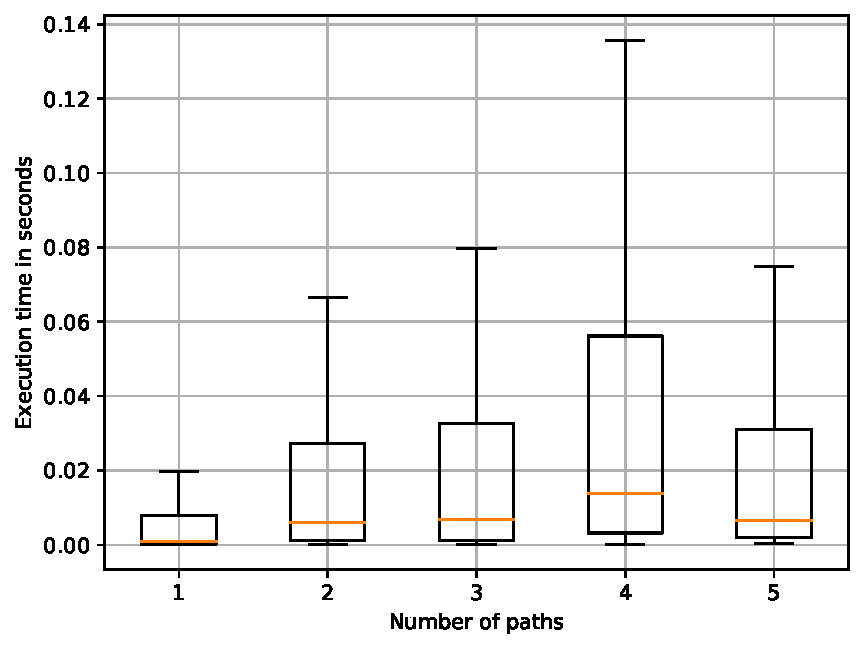
\includegraphics[width=\linewidth,trim=0 0 -1.5cm 0]{pictures/tensor_go_10_small.pdf}
%		\caption{small number of paths} \label{fig:extractTimeGoSmallTns}
%	\end{subfigure}
%	\hspace*{\fill} % separation between the subfigures
%	\begin{subfigure}{0.32\textwidth}
%		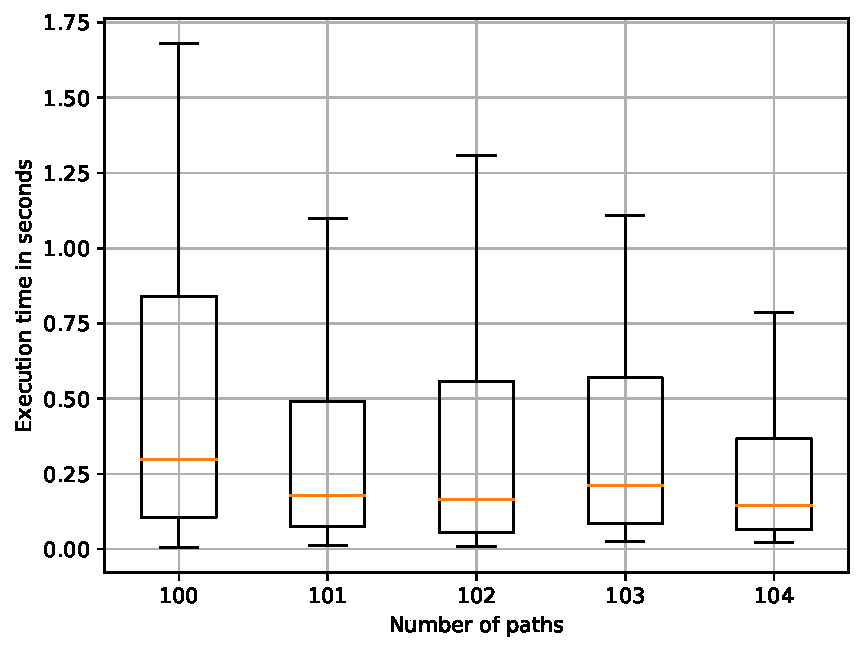
\includegraphics[width=\linewidth,trim=0 0 -1.5cm 0]{pictures/tensor_go_10_big.pdf}
%		\caption{medium number of paths} \label{fig:extractTimeGoMedTns}
%	\end{subfigure}
%	\hspace*{\fill} % separation between the subfigures
%	\begin{subfigure}{0.32\textwidth}
%		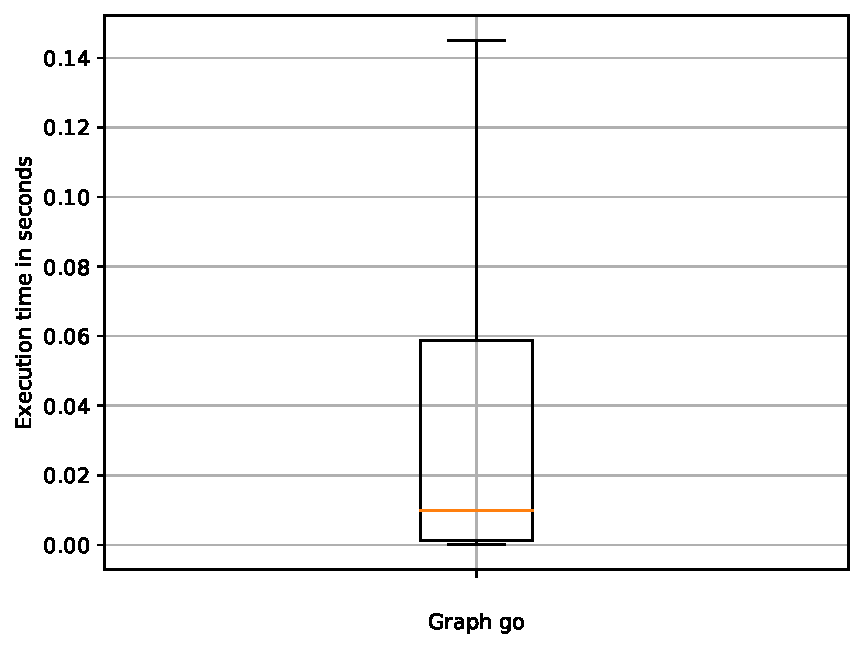
\includegraphics[width=\linewidth,trim=0 0 -1.5cm 0]{pictures/go_10_all_tensor.pdf}
%		\caption{average path extraction time} \label{fig:extractTimeGoAverageTns}
%	\end{subfigure}
%	\caption{Execution time of the Kronecker product-based path extraction algorithm from~\cite{kron} implemented in $Tns$ for the graph $go$}
%	\label{fig:extractTimeTns}
%\end{figure*}

%\begin{figure*}
%	\begin{subfigure}{0.32\textwidth}
%		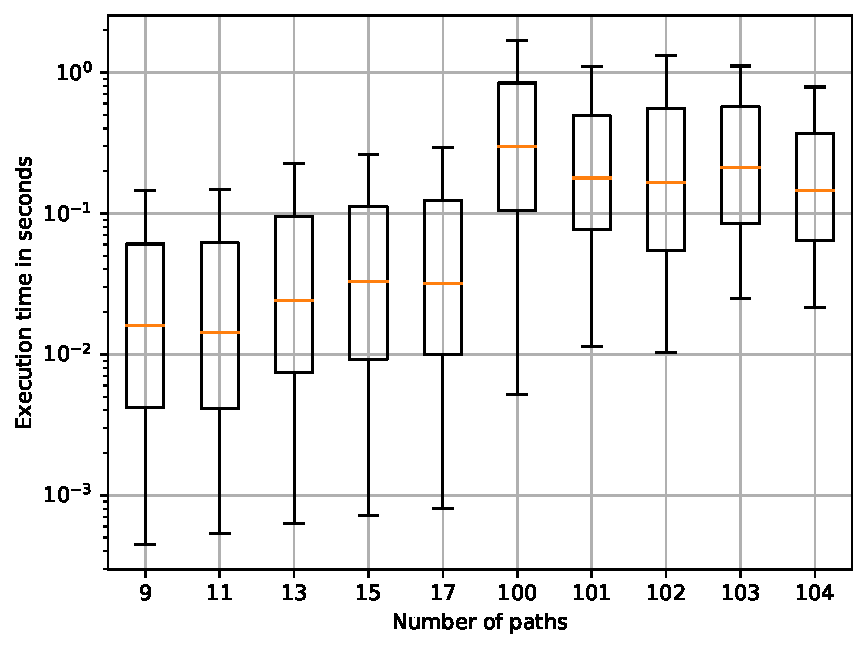
\includegraphics[width=\linewidth,trim=0 0 -1.5cm 0]{pictures/tensor_go_10_big_small.pdf}
%		\caption{$Tns$ path extraction depending on number of paths} \label{fig:extractTimeGoMtx}
%	\end{subfigure}
%	\hspace*{\fill}
%	\begin{subfigure}{0.32\textwidth}
%		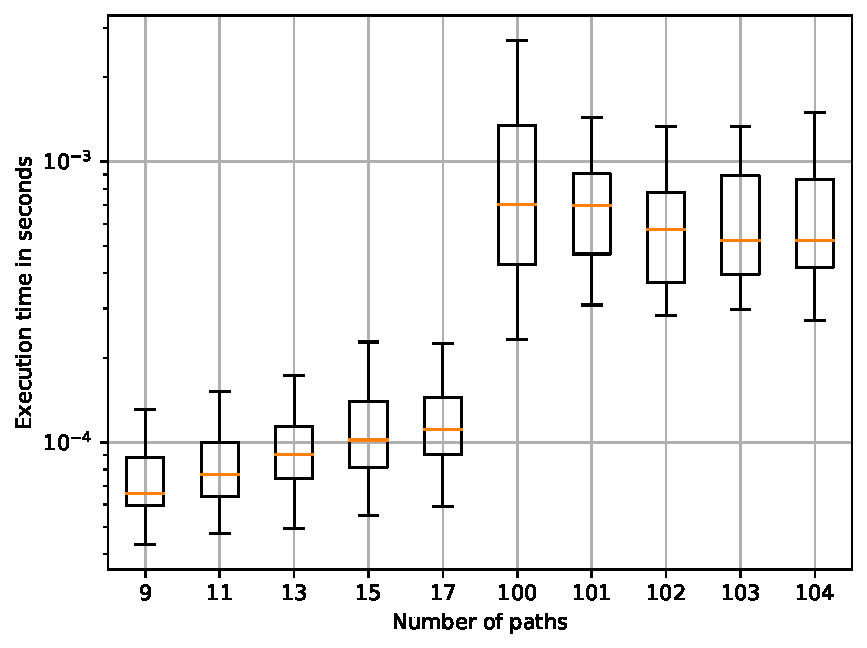
\includegraphics[width=\linewidth,trim=0 0 -1.5cm 0]{pictures/allMatr_go_10_big_small.pdf}
%		\caption{$MtxAll$ path extraction depending on number of paths} \label{fig:extractTimeGoTns}
%	\end{subfigure}
%	\hspace*{\fill} % separation between the subfigures
%	\begin{subfigure}{0.32\textwidth}
%		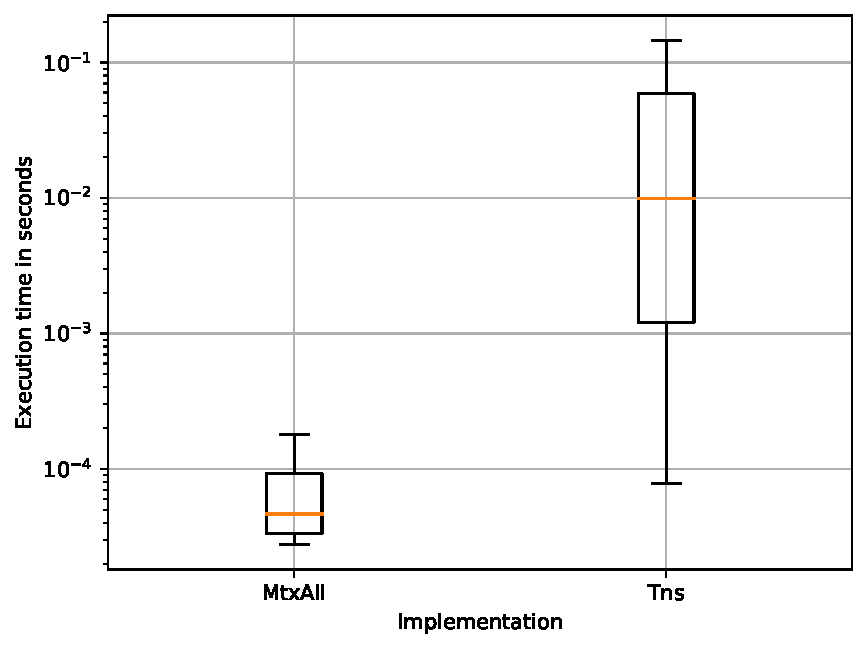
\includegraphics[width=\linewidth,trim=0 0 -1.5cm 0]{pictures/go_10_all_matrixall_tensor.pdf}
%		\caption{average path extraction time} \label{fig:extractTimeGoAverage}
%	\end{subfigure}
%	
%	\caption{Execution time of the proposed matrix-based path extraction algorithm implemented in $MtxAll$ and the Kronecker product-based path extraction algorithm from~\cite{kron} implemented in $Tns$ for the graph $go$}
%	\label{fig:extractTime}
%\end{figure*}

The results of the MCFL-reachability evaluation for queries $Q_1$ and $Q_2$ are presented in Table~\ref{tbl:tableRDF}. We can see, that while the execution time for small graphs is decent, our prototype implementation is underperforming for graphs with thousands of vertices. To show the reason for such behavior, we also present the number of non-zero elements in matrices $B_p$ and $C_p$ added by the MCFL-reachability algorithm in Table~\ref{tbl:tableNNZ}. The $NNZ_1$ is a sum of non-zero elements in these matrices for the query $Q_1$, and the $NNZ_2$ --- for the query $Q_2$. This information describes the big amount of consumed memory and the complexity of the used matrix operations. Our implementation is underperforming for used graphs and queries because there is a big number of combinations of paths that are relevant to the query, and was founded by our algorithm. The used graphs are composed entirely of edges that are relevant to the query, and they form such a large number of combinations. For more practical use of our algorithm, the huge graphs can contain only a small part of the edges that are relevant to the query. This will lead to a decent number of the non-zero matrix elements, a small number of used memory, and a small running time. Also, for big graphs our algorithm constructs matrices of huge sizes that can exceed the numeric range of integer data types. However, this problem can be solved since there are formats like COO (coordinate list) for storing the sparse matrices that stores only non-zero values and does not depend on the matrix size.


{\setlength{\tabcolsep}{0.3em}
\begin{table}[ht]
\centering
\caption{MCFL-reachability execution time in seconds for queries $Q_1$ and $Q_2$}
\label{tbl:tableRDF}
%\rowcolors{1}{}{lightgray}
\begin{tabular}{| c | p{1cm} | c | c | c | c || c | p{1.3cm} | c | c | c | c |}
    \hline
      &  Graph              & \#V & \#E  & $Q_1$  & $Q_2$ &  & Graph & \#V & \#E     & $Q_1$    & $Q_2$ \\
       \hline
       \hline
    \parbox[t]{2mm}{\multirow{5}{*}{\rotatebox[origin=c]{90}{RDF}}}
      & \small{skos}                    & 144 & 323     & 0.07  & 0.08 &
     \parbox[t]{2mm}{\multirow{1}{*}{\rotatebox[origin=c]{90}{}}} & \small{pathways}                    & 6,238 & 37,196  & 533.73 &   148.62   \\\cline{7-12}
      %& \small{generations}                 & 129 & 351     & 0.04  & 0.03 &\parbox[t]{2mm}{\multirow{4}{*}{\rotatebox[origin=c]{90}{LFR}}} & $LFR\_100$& 100 & 210 & 0.03 & 0.04\\
      & \small{pizza}                       & 671 & 2,604    & 3.75  & 2.06 &\parbox[t]{2mm}{\multirow{4}{*}{\rotatebox[origin=c]{90}{LFR}}} & $LFR_{100}$& 100 & 210 & 0.12 & 0.06      \\
      & \small{wine}                        & 733 & 2,450    & 4.55  & 4.41 & & $LFR_{500}$ & 500 & 970 & 2.55 & 1.47      \\
      & \small{funding}                     & 778 & 1,480    & 1.68  & 1.50 & & $LFR_{1000}$ & 1,000 & 2,100 & 13.50 & 6.10      \\
      & \small{core}                        & 1,323 & 8,684   & 10.77  &  9.93 & & $LFR_{10000}$ & 10,000& 21,005 &  1,261.97 & 656.28      \\
      \hline
  \end{tabular}
\end{table}
}

{\setlength{\tabcolsep}{0.3em}
\begin{table}[ht]
\centering
\caption{The number of non-zero elements in matrices after the MCFL-reachability evaluation}
\label{tbl:tableNNZ}
%\rowcolors{1}{}{lightgray}
\begin{tabular}{| c | p{1cm} | c | c | c || c | p{1.3cm} | c | c | c |}
    \hline
      &  Graph               & \#E  & $NNZ_1$  & $NNZ_2$ &  & Graph  & \#E     & $NNZ_1$    & $NNZ_2$ \\
       \hline
       \hline
    \parbox[t]{2mm}{\multirow{5}{*}{\rotatebox[origin=c]{90}{RDF}}}
      & \small{skos}                 & 323     & 5,043  & 5,312 &
     \parbox[t]{2mm}{\multirow{1}{*}{\rotatebox[origin=c]{90}{}}} & \small{pathways}                 & 37,196  & 19,452,226 &   9,734,396   \\\cline{6-10}
      %& \small{generations}                 & 129 & 351     & 0.04  & 0.03 &\parbox[t]{2mm}{\multirow{4}{*}{\rotatebox[origin=c]{90}{LFR}}} & $LFR\_100$& 100 & 210 & 0.03 & 0.04\\
      & \small{pizza}                    & 2,604    & 201,554  & 134,993 &\parbox[t]{2mm}{\multirow{4}{*}{\rotatebox[origin=c]{90}{LFR}}} & $LFR_{100}$ & 210 & 5,687 & 2,851      \\
      & \small{wine}                     & 2,450    & 252,323  & 241,485 & & $LFR_{500}$ & 970 & 118,449 & 63,786      \\
      & \small{funding}                  & 1,480    & 101,304  & 94,401 & & $LFR_{1000}$ & 2,100 & 553,002 & 276,299     \\
      & \small{core}                     & 8,684   & 531,900  &  503,943 & & $LFR_{10000}$ & 21,005&  55,172,204 & 27,349,209      \\
      \hline
  \end{tabular}
\end{table}
}

We conclude that we should improve our implementation to achieve better performance, and find the graphs and queries for more practical use, while the algorithm idea is viable.

%We can see that the most performant index creation is in $MtxRel$ implementation, especially on big graphs. But $MtxRel$ is applicable only for relational query semantics  and cannot restore any paths of interest. Thus, for relational query semantics we can use a more simple index (Boolean matrices) to only solve the reachability problem. The $MtxSingle$ implementation constructs the index up to 2 times slower on big graphs and consumes more memory. This is the cost of storing additional information in the index for the single-path query semantics to be able to restore only one path for each vertex pair. The $MtxAll$ and $Tns$ implementations construct the index up to 2-3 times slower than the $MtxSingle$ implementation and also consumes even more memory, especially on big graphs like $geospecies$ with complex structure for the same-generation query. These two implementations support the all-path query semantics and make it possible to restore all paths corresponding to the same-generation query. However, the Kronecker product-based implementation $Tns$ uses a more complex but compact index and consumes less memory. The implementation $MtxAll$ of the proposed matrix-based CFPQ algorithm for all-path query semantics has comparable execution time to $Tns$  on small graphs but $MtxAll$ is significantly slower and consumes more memory on some big graphs with complex structure than $Tns$. The reason for such behavior is that the proposed matrix-based algorithm is trying to store the information of all founded paths more explicitly, and the index constructed by $MtxAll$ is less compact than the one constructed by $Tns$.

	


%After constructing the index, we compared the execution time of the path extraction for CFPQ with all-path query semantics using both $MtxAll$ and $Tns$ implementations. The results of path extraction for graph $go$ are presented in Figure~\ref{fig:extractTime} (boxplots are standard, medians are indicated and outliers are omitted). For computation termination, we limit the maximum path length to 10 since most of the paths of interest in the graph $go$ satisfy this constraint. After that, we extract paths for each vertex pair and group the execution time by the number of paths returned in Figures~\ref{fig:extractTimeGoMtx} and \ref{fig:extractTimeGoTns} (not all number of paths are presented). Also, we provide the average path extraction time for both implementations and graph $go$ in Figure~\ref{fig:extractTimeGoAverage}. Note that the global medians in Figure~\ref{fig:extractTimeGoAverage} are lower than all the respective medians shown in the Figures~\ref{fig:extractTimeGoMtx} and \ref{fig:extractTimeGoTns} since there are many vertex pairs in the graph $go$ with the number of found paths less than 9. We can see that the path extraction running time of the implementation $MtxAll$ of the proposed matrix-based algorithm is up to 1000 times faster than for the Kronecker product-based implementation $Tns$. As was mentioned above, in the proposed matrix-based CFPQ algorithm we construct an index with more explicit information about all paths found. Thus, paths can be restored significantly faster than using the Kronecker product-based algorithm.

%We can conclude the following.
%\begin{itemize}
	%\item %Our evaluation allows us to conclude that the most performant linear algebra-based algorithm for the CFPQ with relational and single-path query semantics are matrix-based algorithms from~\cite{Azimov:2018:CPQ:3210259.3210264} and \cite{10.1145/3398682.3399163} respectively.
	%\item %For all-path query semantics, the proposed matrix-based and the Kronecker product-based CFPQ algorithms have the following tradeoffs. If it is necessary to frequently recalculate the index for a changing graph or a path query then the best choice is the Kronecker product-based algorithm~\cite{kron} with faster and less memory consuming index construction. If it is necessary to extract paths many times for a once constructed index or index changes can be efficiently computed dynamically then the proposed matrix-based CFPQ algorithm is preferable.
%\end{itemize}



